\chapter{Adapting Real World Objects for Custom Users and Use Cases}

In our everyday life, we often find a need to adapt objects or tools, as the way they were originally designed might not work for certain users or use cases. For example, a faucet might be out of reach for a child, thus it needs to be extended\footnote{\url{http://peachyco.com/handleextender.html}} (Figure~\ref{fig:reprise_existing_adaptations}a); it is hard to hold a drill bit straight while sharpening it, thus a guide comes in handy to keep it in place\footnote{\url{http://www.thingiverse.com/thing:1024834}} (Figure~\ref{fig:reprise_existing_adaptations}b); painting a big surface with a spray-can could be fatiguing for the fingers, thus a mechanism can be used to turn it into a spray-gun\footnote{\url{http://www.thingiverse.com/thing:51966}} (Figure~\ref{fig:reprise_existing_adaptations}c). These add-on components are called \textit{adaptations}. Adaptations change the mechanical properties of existing objects to make them more accessible or to customize them for specific use cases.

The advent of low-cost 3D printing offers the possibility to rapidly construct a wide range of adaptations. However, designing or re-purposing adaptations is hard with general-purpose 3D modeling software, as it requires a certain level of expertise from users \cite{hurst2013making}. In general, 3D modeling tools do not take into account how an object is used, what adaptation strategy is available, or how to rapidly generate the corresponding geometry or further customize it.

Prior work, such as Patching \cite{teibrich2015patching}, Encore \cite{chen2015encore} and AutoConnect \cite{koyama2015autoconnect}, mostly focuses on attaching or directly fabricating new components onto existing objects. However, it remains unclear how to design these components so that they can serve to adapt the objects in user-customized ways. P.Pod \cite{davidoff2011mechanical} and RetroFab \cite{ramaker2015retrofab} explored the mechanical problem of hijacking and automating controls on existing physical interfaces. However, such mechanisms are usually too heavyweight for adapting common household items and hand tools. 

In this chapter, I build on previously explored attachment techniques, and develop a design tool for specifying, generating, customizing and fitting 3D printable adaptations onto everyday objects. My particular focus is on empowering end users to leverage new fabrication technologies to create adaptations by providing high-level techniques for specification and computational support for geometry generation.

Reprise allows a user to specify how an object is used and with what types of action, such as using a virtual hand (Figure~\ref{fig:reprise_teaser}b) to indicate how a person would hold a wire cutter. As 3D geometry itself does not encode how an object is used in the real world, Reprise' techniques enable a user to interactively describe this information \textit{in situ} on models of the objects.

Once the actions are specified, this information is fed into a library of design strategies--Wrapper/Extension, Handle, Lever, Anchor/Stand, and Guide (Figure~\ref{fig:reprise_design_space}). These adaptation strategies were derived from an analysis of over 3000 lifehacking and assistive technology examples found in three books \cite{plaxen2005adapt, willkolmm2013assistive, robitaille2010illustrated} and two online communities \cite{thingiverse,pinterest}. A user can select one or more strategies, which automatically generate the initial design of an adaptation, such as a wrapper for a cutter's handle (Figure~\ref{fig:reprise_teaser}c), levers for easing  clutching operation (Figure~\ref{fig:reprise_teaser}g), or a structure to anchor the cutter for situated use (Figure~\ref{fig:reprise_teaser}i).

To further iterate on the design, a user can manipulate simple slider widgets to customize these adaptations to better suit the person's needs and preferences, such as making the cutter's wrapper longer and thicker for easier gripping (Figure~\ref{fig:reprise_teaser}d), increasing the levers' torque for clutching (Figure~\ref{fig:reprise_teaser}g), or making a larger base for stability (Figure~\ref{fig:reprise_teaser}k). Finally, Reprise also provides a simple toolkit for making the adaptations more attachable onto the objects, such as generating a pipe clamp that connects the cutter's handle to the anchor (Figure~\ref{fig:reprise_teaser}k).

\begin{figure*}
  \centering
  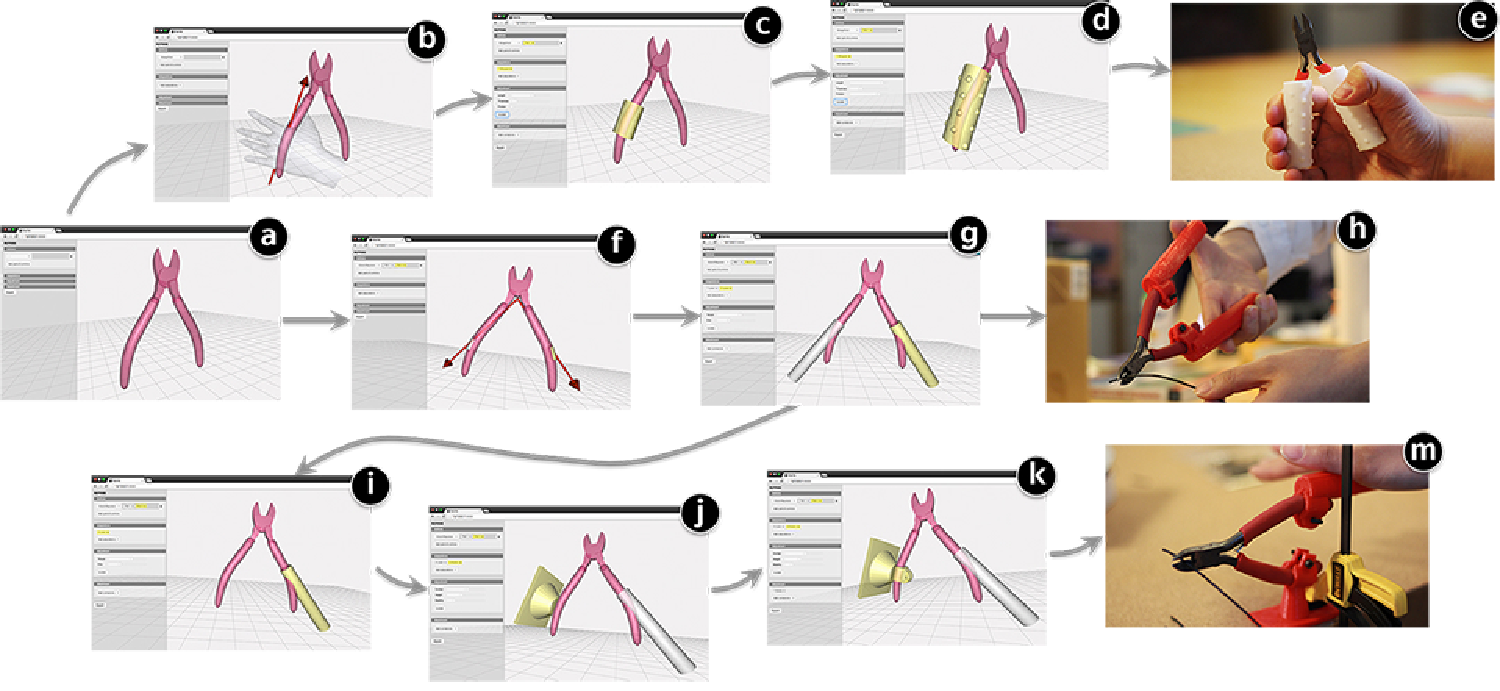
\includegraphics[width=1\textwidth]{figures/reprise_scenarios_v1.pdf}
  \caption{Our main contribution is the tool integration and a formalized design workflow for making 3D printable adaptations onto everyday objects. For example, an occupational therapist can use our tool to explore different strategies of adapting a wire cutter (a), such as creating a wrapper to soften the grip (b-e), adding two levers to assist with clutching (f-h), or replacing one lever with an anchor to situate the cutter on the work surface (i-m).}~\label{fig:reprise_teaser}
\end{figure*}

To demonstrate the expressiveness as well as understanding the limitations of Reprise, we replicated existing adaptation examples found during our design space exploration (Figure~\ref{fig:reprise_design_space}). We identified a real world exemplar for each of 18 cells of the two-dimensional design space. Among the 18 examples, Reprise was able to replicate 15 of them; the other 3 cases suggest new features to be added to the tool and  fertile opportunities for future work.

\begin{figure}[!h]
  \centering
  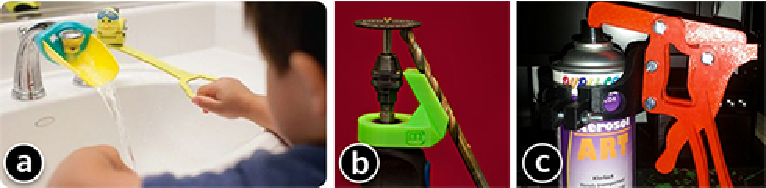
\includegraphics[width=0.7\textwidth]{figures/reprise_existing_adaptations.pdf}
  \caption{Existing examples of adapting everyday objects: a faucet extension (a), a guide for sharpening drill bit (b), and turning a spray-can to a spray-gun (c).}~\label{fig:reprise_existing_adaptations}
\end{figure}

The main contribution of the Reprise tool lies in its ability to generate and iterate across a range of likely useful adaptations. However, it can also be seen as an early exemplar in a class of design tools which can make 3D printing more accessible and useful for ordinary people. In particular, it goes beyond the specification of geometry alone to provide very application domain specific knowledge and features.  This helps to substantially reduce the gulf of execution \cite{norman2013design} that users must bridge as they cross from function to geometry, e.g., from geometric form to the implications of that geometry on the desired end result.

\section{Scenario Walkthrough: Adapting a Cutter}
Reprise lets a user explore a range of design strategies for adapting everyday objects. To set the scene, we first walk through the flow of Reprise in an exemplar scenario where Larry--an occupational therapist--is trying to adapt a wire cutter for an electrician who recently suffered from a hand injury.

\subsection{Iteration I: Generating Wrappers for a Better Grip}
To start, Larry imports a 3D model of the cutter (from a provided repository or through scanning). He selects `Grasp/Hold' as the type of action the patient is having difficulty with. He then clicks on the handle of the cutter to specify the part that is being grasped. Reprise shows a virtual hand model, which Larry can rotate to indicate the relative orientation between the gripping hand and cutter (Figure~\ref{fig:reprise_teaser}b). Next, Larry selects `Wrapper/Extension' as the adaptation strategy. Based on the previously specified grasping action and its hand orientation, the system generates an initial design of the wrapper (Figure~\ref{fig:reprise_teaser}c). Larry wants to further tweak the design using simple slider controls. He adjusts the `Length' slider to make sure the wrapper covers an area large enough for three fingers. He then increases the thickness to make a rounder grip. To further tighten the grip, he adds small bumps to increase the friction (Figure~\ref{fig:reprise_teaser}d). Finally, Larry exports the generated geometry as an STL file and prints the adaptation using a soft material (such as NinjaFlex\footnote{\url{http://www.ninjaflex3d.com/products/ninjaflex-filaments/}}), which provides a soft grip and makes the wrapper snugly fit with the cutter's handle (Figure~\ref{fig:reprise_teaser}e).

\subsection{Iteration II: Making Levers to Assist with Clutching}
Larry's patient responds positively to the soft wrapper. However, while he can now comfortably hold the cutter, his hand is still too weak to perform the necessary clutching action, especially when cutting hard wires. Thus Larry explores an alternate design strategy. In Reprise, he first selects `Clutch/Squeeze' as the target operation. He selects the two handles as the components on which clutching is applied, and then moves the cursor to indicate the fulcrum of clutching. In these few steps, he specifies the two arms for clutching (Figure~\ref{fig:reprise_teaser}f). With this information, Larry proceeds to select `Lever' as the adaptation strategy, which automatically generates two levers from the handles (Figure~\ref{fig:reprise_teaser}g). Larry then tweaks the design, playing with the torque of the levers, as well their size for grasping.

\subsection{Iteration III: Anchoring the Cutter for Situated Use}
Larry's patient does not like the lever design, as it  makes the cutter somewhat too big to hold in one hand (Figure~\ref{fig:reprise_teaser}h). To solve the problem, Larry uses Reprise to replace one lever with an anchoring structure with which he can affix one of the cutter's handles on the work surface (Figure~\ref{fig:reprise_teaser}ij). The patient then simply uses his palm and body weight to press down and cut wires. The key here is to firmly attach the anchor to the cutter's handle. Reprise's attachment toolkit allows Larry to generate a pipe clamp for holding the cutter in place on the anchor (Figure~\ref{fig:reprise_teaser}k). Once printed, Larry bolts the cutter on the anchor, which is then clamped onto the patient's work surface (Figure~\ref{fig:reprise_teaser}m).

To summarize, Reprise allows Larry to generate adaptations with just a few clicks, to tweak the design using simple slider controls, and to explore different design strategies while iterating and customizing the adaptation to suit the patient's particular needs and preferences. Below we describe a design space that informs the design and implementation of Reprise.

\begin{figure*}[!p]
  \centering
  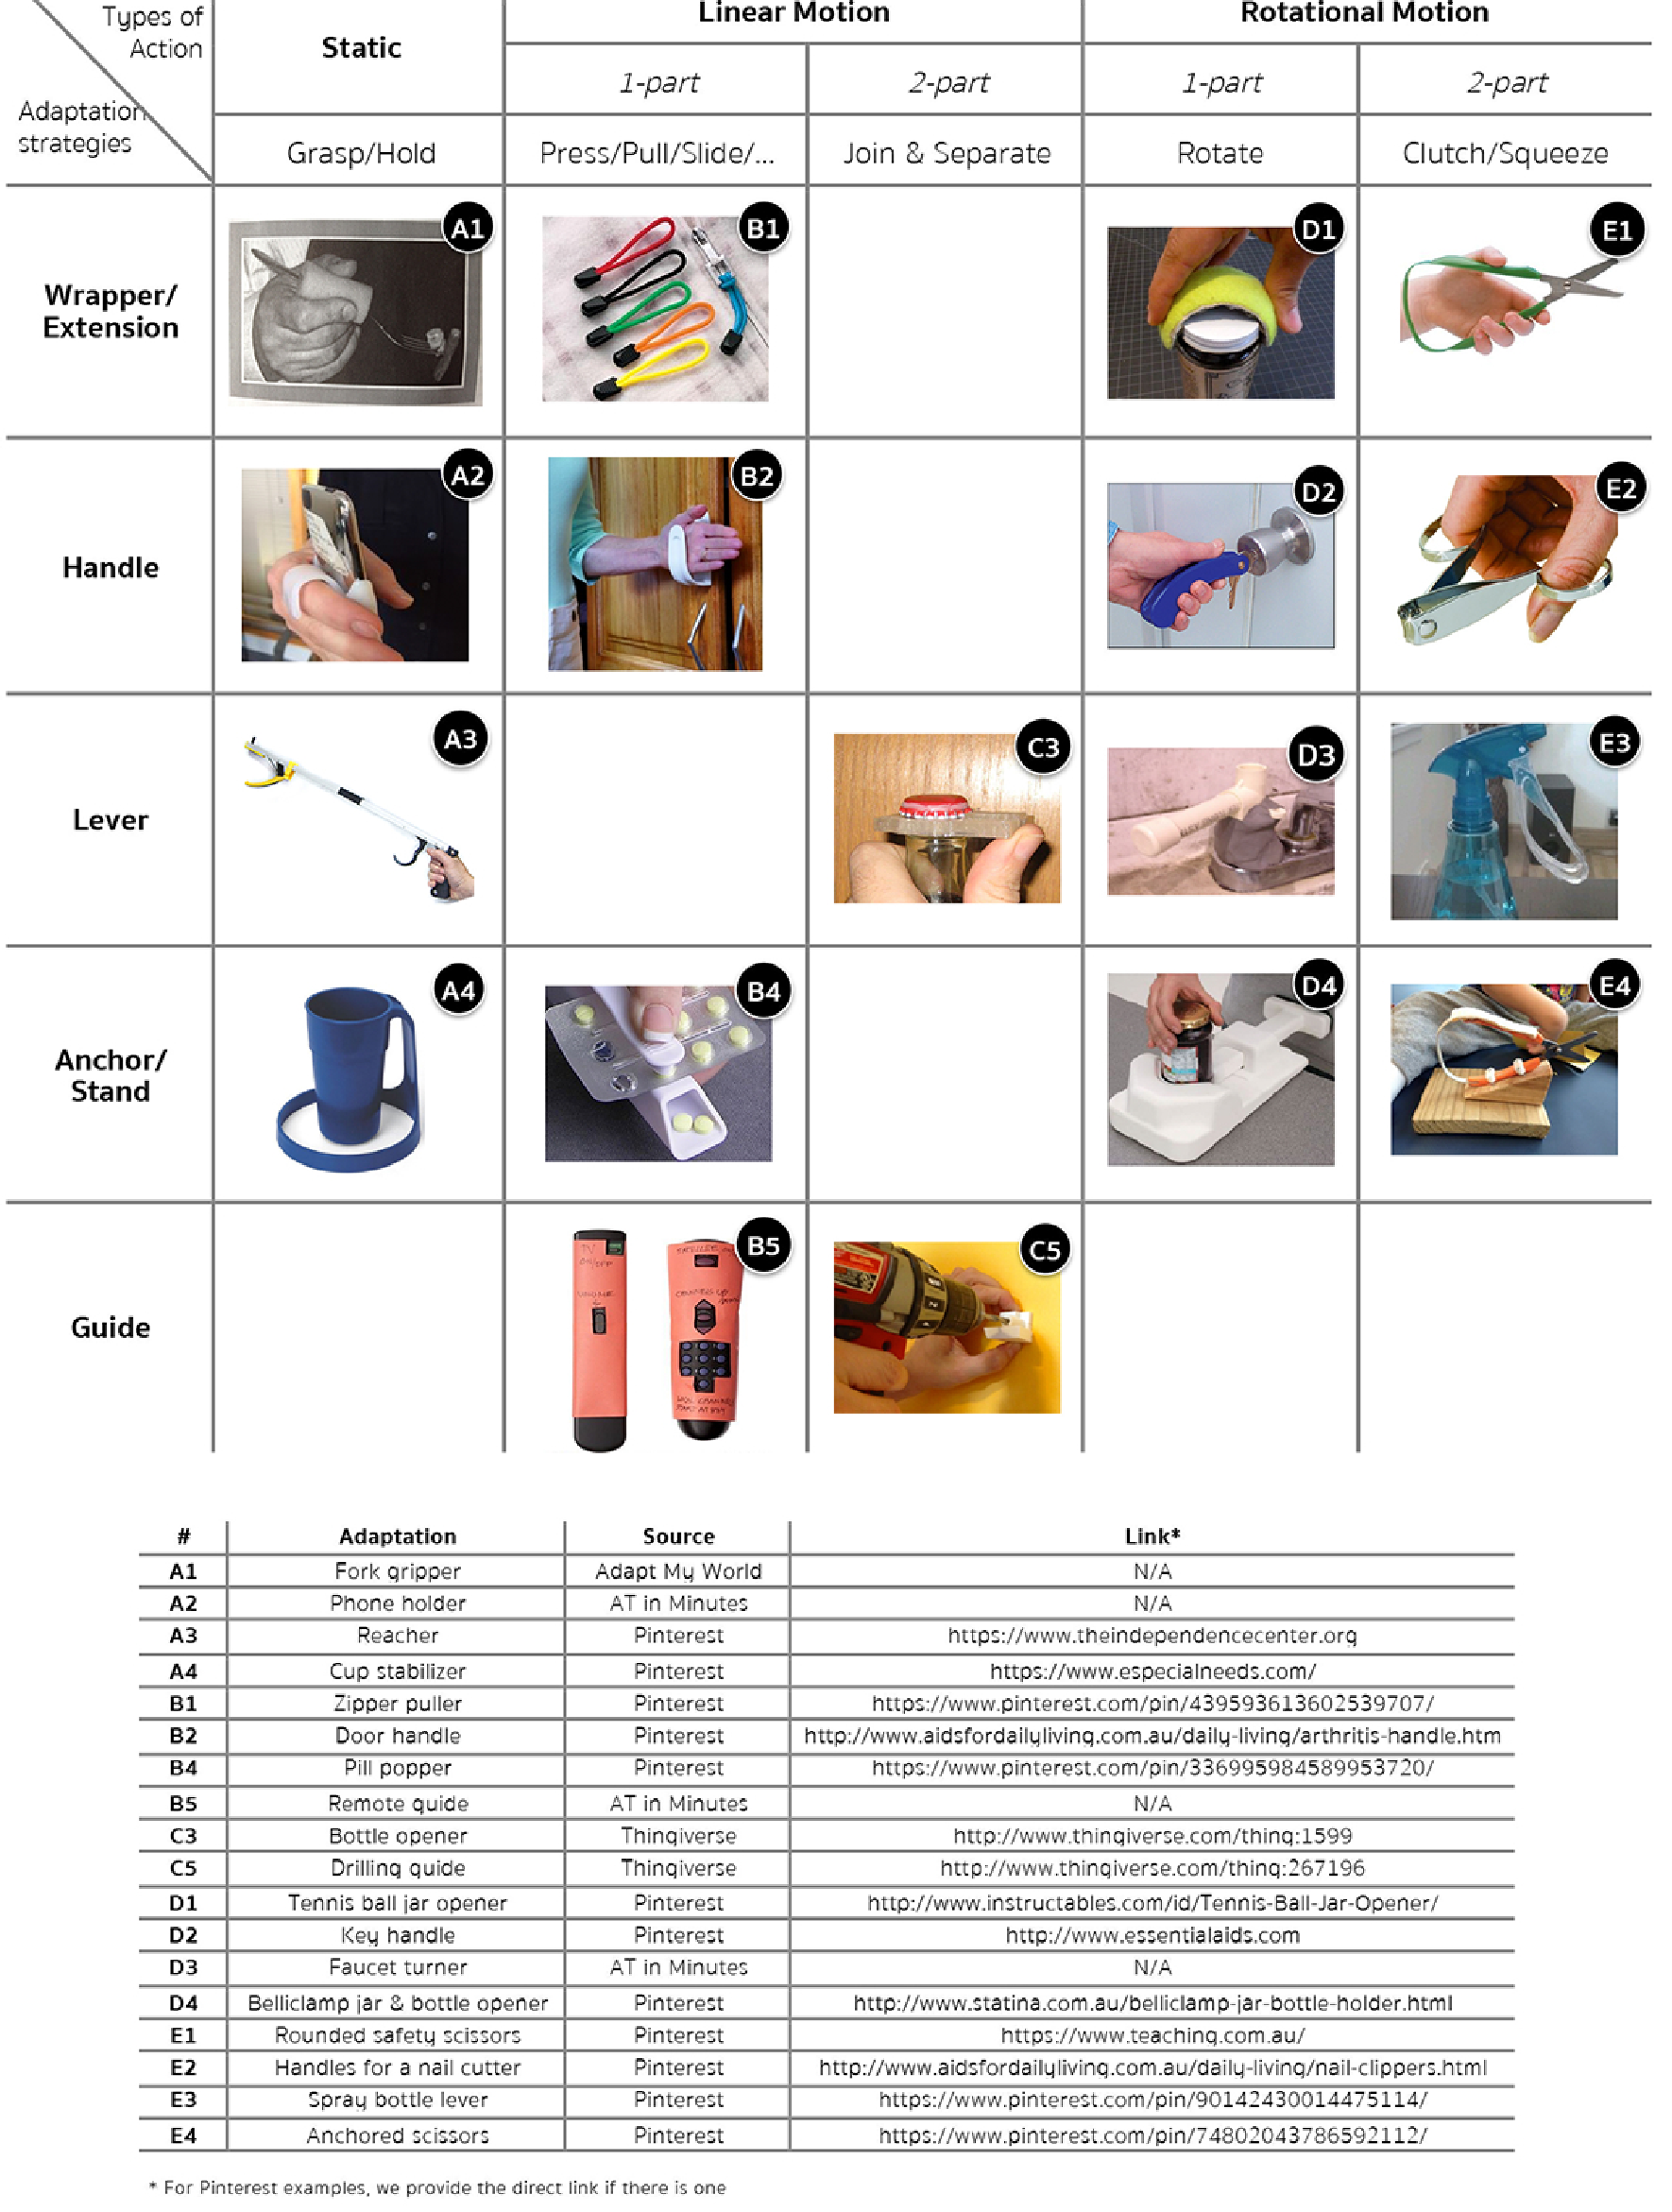
\includegraphics[width=0.9\textwidth]{figures/reprise_adaptation_design_space_v2.pdf}
  \caption{A design space of adaptations summarized from over 3000 existing examples: five major adaptation strategies support various types of actions, from static grasp and hold, to linear and rotational motion that involves one or multiple parts of the objects.}~\label{fig:reprise_design_space}
\end{figure*}

\section{A Design Space of Adaptation Strategies}
For years, well before digital fabrication was widespread, people have been taking a `bricolage' approach for making adaptations on objects that would otherwise be difficult to use. In particular, many innovative solutions came from the need to create assistive technologies (AT) for people with special needs. For example, Werner documented his effort in making assistive technology for village children with very limited resources \cite{werner1987disabled}. Books like \cite{plaxen2005adapt, willkolmm2013assistive, 9781933940021} have compiled simple recipes for individuals to adapt household items and tools with materials that can easily be found at home. Although started with a small and specific audience, these AT design and making solutions usually have a broader impact and implication on universal design \cite{de2011design}. 

Another source of inspiration is online communities such as Thingiverse \cite{thingiverse} and Pinterest \cite{pinterest}, which curate a repertoire of lifehacking solutions people have explored and shared with one another. Recent work by Buehler et al. \cite{buehler2015sharing} has summarized a plethora of assistive technology from Thingiverse, which suggests promising opportunities of learning from these resources.

To inform the computational design of adaptation, we collected and reviewed over 3000 lifehacking and assistive technology examples from the aforementioned literature (85 from \cite{plaxen2005adapt}, 56 from \cite{willkolmm2013assistive}, and 33 from \cite{robitaille2010illustrated}) and online communities (950 from Pinterest  and 2028 from Thingiverse using queries `assistive', `technology' and `adaptation'). Amongst these examples, we identified adaptation designs, and  organized them into themes in a bottom-up fashion. This sampling process continued until we felt that we had reached saturation.

% Rather than attempting to exhaust all possible assistive technology, our goal here was to follow a bottom-up approach: building up a large body of examples, filtering them with a focus on adaptation, and summarizing the findings to inform the design of Reprise.

We present our findings as a design space of adaptation strategies. As shown in Figure~\ref{fig:reprise_design_space}, we identified five major categories of adaptation designs, as well as the types of actions they support to hold, control or operate the objects. While some examples might fit in multiple categories, this design space captures the range of ideas we found in our review and suggests opportunities for novel adaptations (which we discuss in the Results section).

\textbf{\#1 Wrapper/Extension} is something wrapped around an existing object or an extension that lengthens or expands it. Wrapper and extension support various actions with objects. A wrapper can be used to soften the grip (A1), or to assist with grabbing and rotating an object  with less force or less fine motor control (D1). An extension can help with pulling an object (B1) or--with a specific design--to enhance safety for cutting tools (E1).

\textbf{\#2 Handle} is an add-on grippable part attached to an existing object, which makes the object easier to hold (A2), pull (B2), or rotate (D2). Adding handles also helps with clutching, such as using a nail cutter (E2).

\textbf{\#3 Lever} is a structure added to an existing object, usually to make it easier to be turned or rotated, such as the lever used in D3 for turning a faucet, or in E3 for squeezing a spray bottle. In other cases, a lever also affords actions other than rotation, such as grabbing objects (A3), or opening a beer bottle (C3).

\textbf{\#4 Anchor/Stand} is a structure with which an existing object can be stably situated or affixed to the environment. Figure~\ref{fig:reprise_design_space} shows a stand to hold the cup stable (A4), a pill popper for holding a pack of pills and popping them out (B4), a clamp for holding a jar or bottle for easier opening (D4), and an anchor for a pair of scissors for situated use (E4).

\textbf{\#5 Guide} is a structure that guides the movement of, or against, certain objects or their components. B5 shows a guide for locating and pressing buttons on remote controls. C5 is a guide for drilling a screw vertically towards and into a surface. 

Having summarized these five major adaptation strategies, below we describe the technical details of Reprise--a tool that integrates and implements these strategies for generating 3D printable adaptations.

\begin{figure*}
  \centering
  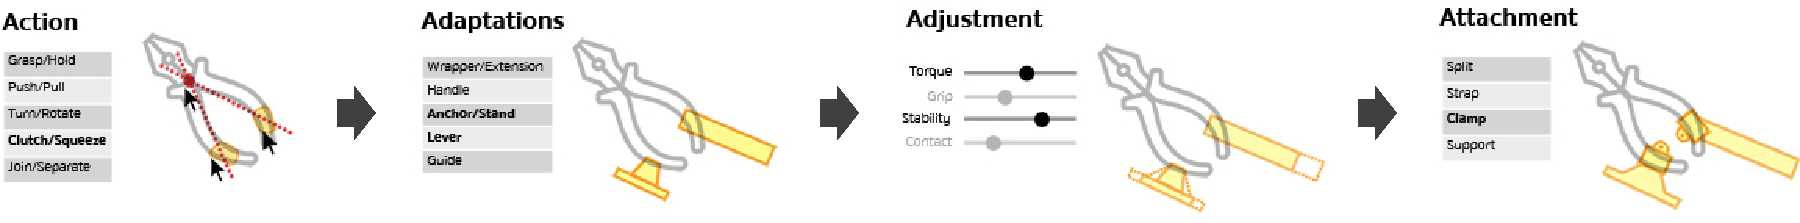
\includegraphics[width=1\textwidth]{figures/reprise_sys_overview_v1.pdf}
  \caption{The design workflow of Reprise. Start with specifying the types of \textit{action} applied on an object, which serves as input for generating user-selected \textit{adaptations}. The initial design can be further customized by \textit{adjusting} a set of parameters. Finally, extra fasteners can be added to make adaptations more \textit{attachable} onto the object.}~\label{fig:reprise_sys_overview}
\end{figure*}

\section{Reprise: Computational Design of Adaptations}
Figure~\ref{fig:reprise_sys_overview} shows the workflow of Reprise. Users start with importing a 3D model of an object they want to adapt, specify what types of action is applied, and on which parts of the object. Next they select an adaptation strategy from a library provided by Reprise, which automatically generates the geometry. This initial design can then be customized by adjusting a set of parameters. Finally, extra fasteners can be added to better attach the adaptations onto the object. Reprise then exports all the generated geometry as 3D printable STL files.

\subsection{Techniques for Specifying Types of Action with an Object}
As a user selects a type of action, Reprise provides interaction techniques for specifying where and how the action is applied on the object. As 3D geometry itself does not encode how an object is used in the real world, Reprise's techniques enable the users to specify this information \textit{in situ}, which later serves as input parameters for generating adaptations. Most of these techniques--as described below--start with the user selecting one ore more \textit{points of action}--the locations on the object where it will be held, controlled, or manipulated.

\textbf{Grasp/Hold} As shown in Figure~\ref{fig:reprise_grasp}, Reprise displays a virtual hand, which can be rotated by moving the mouse cursor around the point of action. This allows users to describe the relative orientation between the grasping hand and the object, such as forming a cylindrical grasp \cite{9780323033848} on a fork (Figure~\ref{fig:reprise_grasp}a), or a spherical grasp \cite{9780323033848} on the cap of a water bottle (Figure~\ref{fig:reprise_grasp}b). Reprise also provides a simple jig (Figure~\ref{fig:reprise_hand_measuring}) for measuring the target user's hand size, which can then be entered into the system.

\begin{figure}[h!]
  \centering
  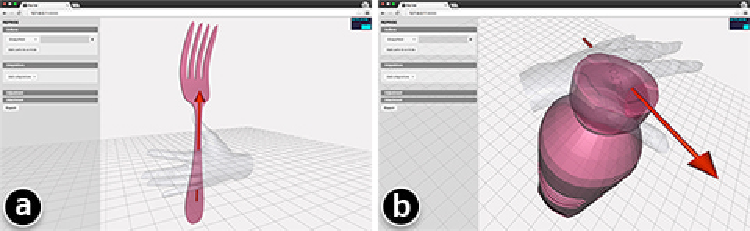
\includegraphics[width=0.75\textwidth]{figures/reprise_grasp_v1.pdf}
\caption{Reprise shows a virtual hand to let the user specify how an object is grasped, such as forming a cylindrical grasp on a knife (a), or a spherical grasp on a bottle (b).}~\label{fig:reprise_grasp}
\end{figure}

\textbf{Push/Pull} A spherical control is used to let the user specify the direction of the push/pull, such as pressing a small power button on a remote (Figure~\ref{fig:reprise_pushpull}a), or pulling a zipper pull horizontally (Figure~\ref{fig:reprise_pushpull}b).

\begin{figure}[h!]
  \centering
  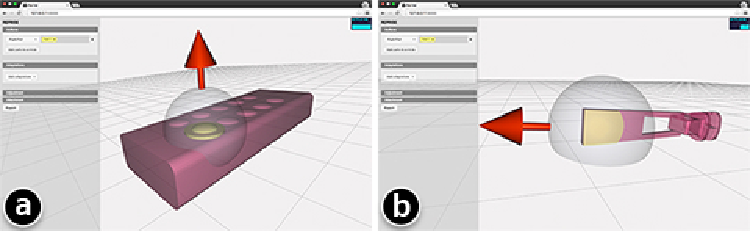
\includegraphics[width=0.75\textwidth]{figures/reprise_pushpull_v1.pdf}
  \caption{Reprise uses a spherical control for specifying pushing/pulling an object, such as pressing a button on a remote control (a), or pulling a zipper (b)}~\label{fig:reprise_pushpull}
\end{figure}

\textbf{Rotate} The user selects the plane ($XY$, $YZ$ or $ZX$) on which the object is rotated, such as the vertical plane on which to turn a door handle (Figure~\ref{fig:reprise_rotate}b). Next the user selects the fulcrum (Figure~\ref{fig:reprise_rotate}c) within that plane. Reprise dynamically displays an arrow pointing from the fulcrum to the point of action to help the user specify the rotating arm (shown as the arrow).
\vskip 5pt

\begin{figure}[h!]
  \centering
  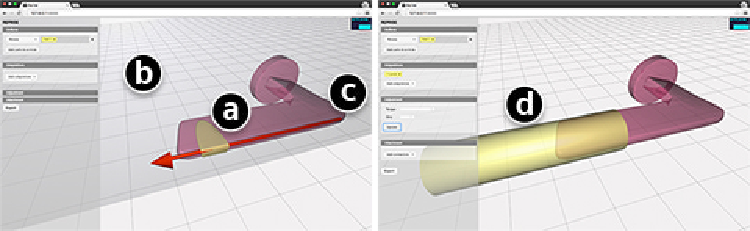
\includegraphics[width=0.75\textwidth]{figures/reprise_rotate_v2.pdf}
  \caption{To specify rotating an object, Reprise lets a user select where the object is held (a), on which plane it is rotated (b), and the fulcrum of rotation (c). The red arrow shows the rotation arm along which a lever can be generated (d).}~\label{fig:reprise_rotate}
\end{figure}

\textbf{Clutch} usually involves two components, such as clutching the two handles of a cutter. Thus the user will select two points of action on the object, such as the handle and the neck of a spray bottle. The plane of clutching is then computed from the normals of the selected points as well as the line segment formed between them. Similar to Rotate, the user then selects a fulcrum on that plane where two arrows are shown indicating the directions of the clutching arms ((Figure~\ref{fig:reprise_clutch}a).

\textbf{Join/Separate} involves two objects moving towards or away from each other. To simplify the problem, Reprise uses their bounding boxes to describe how the objects will be joined or separated. Specifically, the user will select two faces, respectively, from the two bounding boxes, which then shows the direction along which the two objects will moved towards or away from one another. For example, as shown in Figure~\ref{fig:reprise_joinseparate}a, the key would go into the lock hole along its teeth as indicated by the arrows.

\begin{figure}[t]
  \centering
  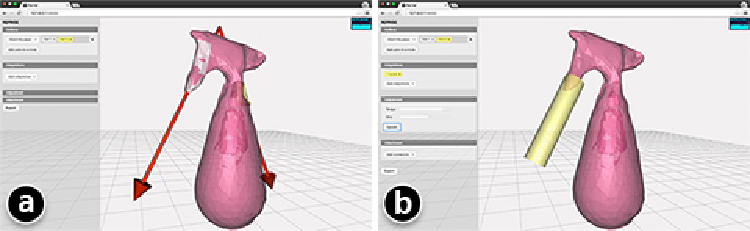
\includegraphics[width=0.75\textwidth]{figures/reprise_clutch_v1.pdf}
  \caption{To specify clutching, the user selects the two parts of the object that are being clutched and then the fulcrum. The red arrows indicate the directions of the clutching arms (a). The user can generate a lever for clutching the spray bottle, while holding its body in hand (b).}~\label{fig:reprise_clutch}
\end{figure}

\begin{figure}[t]
  \centering
  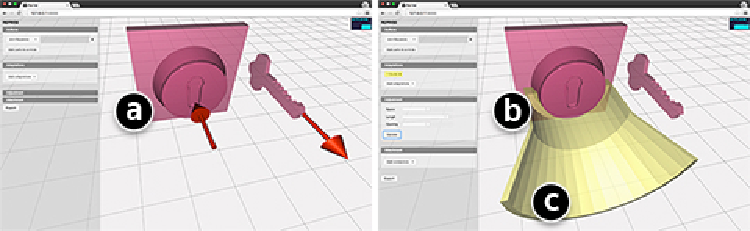
\includegraphics[width=0.75\textwidth]{figures/reprise_joinseparate_v1.pdf}
  \caption{Reprise lets the user specify moving one object towards or away from another, such as putting a key into a lock hole.}~\label{fig:reprise_joinseparate}
\end{figure}

%It is also possible to specify more than one action with an object. For example, for the spray bottle in Figure~\ref{fig:reprise_clutch}, one can also specify a secondary action of `Grasp/Hold' around neck of the bottle.

\subsection{Computationally Generating Adaptations}
Taking the user-specified actions as input parameters, Reprise then provides a list of strategies for rapidly generating the initial design of adaptations. The specific methods for generating these models are based on the aforementioned survey of existing adaptation examples (Figure~\ref{fig:reprise_design_space}). In generating these adaptations, Reprise uses variations of a cylindrical geometry as the primary building blocks, and a series of Constructive Solid Geometry (CSG) operations for creating the specific adaptations. 

\begin{figure}[b]
  \vskip 5pt
  \centering
  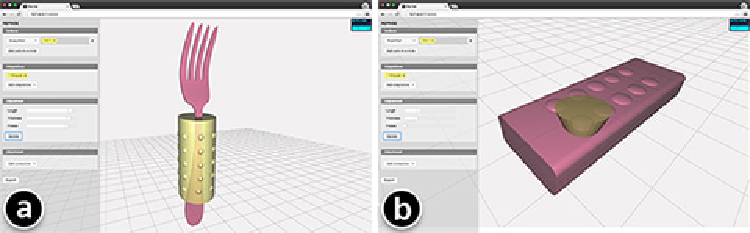
\includegraphics[width=0.75\textwidth]{figures/reprise_wrapper_v1.pdf}
  \caption{Reprise can generate a wrapper--a cylindrical structure bounding part of an object (a), or an extension--an extrusion from a selected area of the object (b).}~\label{fig:reprise_wrapper}
\end{figure}

For example, a cylinder wrapping around part of an object can make a wrapper (Figure~\ref{fig:reprise_wrapper}a) or a lever (Figure~\ref{fig:reprise_rotate}b and Figure~\ref{fig:reprise_clutch}b). Extruding a cylindrical structure from an object's surface creates an extension, such as enlarging a button on a remote control (Figure~\ref{fig:reprise_wrapper}b). To make an anchor, Reprise creates a cylindrical pillar that connects to a rectangular base at the bottom, and to the object at the top (Figure~\ref{fig:reprise_pipeclamp}a). When creating a guide, it is also possible to use an object's bounding cylinder to represent its path of movement, which creates a `tunnel' (Figure~\ref{fig:reprise_joinseparate}b) with a wide `opening' at the entrance (Figure~\ref{fig:reprise_joinseparate}c). By default Reprise displays the models in 1:1 scale to let the user get a concrete sense of the adaptations' size and dimensions when adjusting these parameters.

\subsection{Adjusting Design Parameters for Customization}
With the initial design of the adaptations, Reprise provides users with simple slider controls to adjust the design parameters for further customization. For example, for gripping, they can lengthen a wrapper so that it can be held by multiple fingers (the sizes of which can be measured using a tool described later in Figure~\ref{fig:reprise_hand_measuring}); they can also adjust the radii of the cylindrical components, or add small bumps on the surface to tighten the grip (Figure~\ref{fig:reprise_wrapper}a). To enhance strength and support, they can increase the torque of the levers, or give the anchor or stand a larger base. For easier hand coordination, they can widen the opening in a guide, making it easier to move one object into the `tunnel' and towards the other object (Figure~\ref{fig:reprise_joinseparate}c). To adjust the overall size, they can make a handle more elliptic or vary the length of its arc (Figure~\ref{fig:reprise_all_designs}c).

To help users navigate the rich parameter space, Reprise also allows them, with one click, to generate a large set of design variations (Figure~\ref{fig:reprise_all_designs}a$\rightarrow$b), similar to the technique in Side Views \cite{terry2002side}. This provides them with a more intuitive way of browsing and comparing different designs, select one that best matches what they have in mind (Figure~\ref{fig:reprise_all_designs}b$\rightarrow$c), and from which they can continue to customize the model (Figure~\ref{fig:reprise_all_designs}c). For example, as shown in Figure~\ref{fig:reprise_all_designs}, to make an adaptation for grasping a fork, the user can select wrappers of different length, thickness, and tightness, as well as handles of different sizes and styles.

\begin{figure}[h!]
  \vskip 5pt
  \centering
  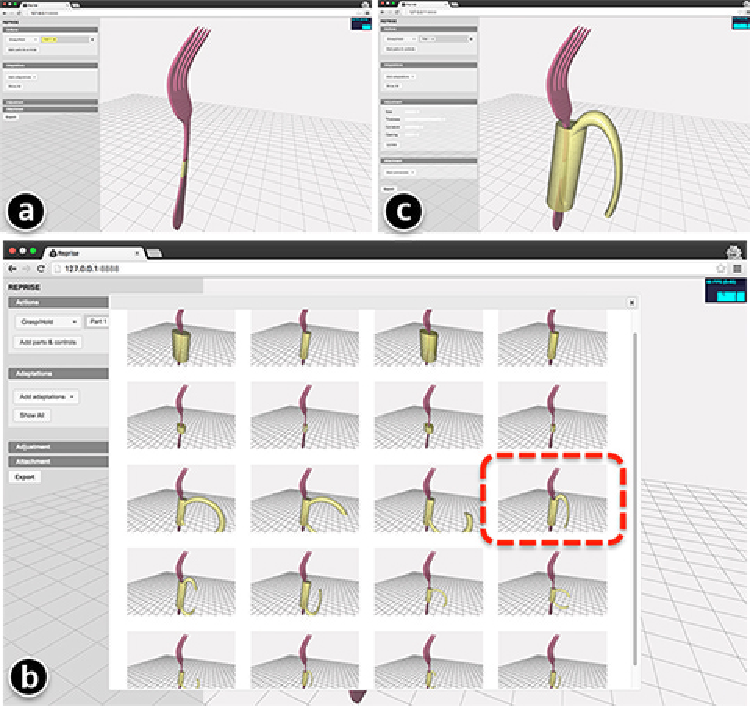
\includegraphics[width=0.75\textwidth]{figures/reprise_all_designs_v2.pdf}
  \caption{Besides using sliders, users can also click a button to generate a large set of design variations (ab), from which they can select one that best matches the design they have in mind, and continue to develop it from that model (c).}~\label{fig:reprise_all_designs}
\end{figure}

\subsection{Attaching Adaptations onto Real World Objects}
As a last step, the user normally wants to generate some attaching mechanism(s) for installing the adaptations onto the object. Prior work, such as Encore \cite{chen2015encore} and AutoConnect \cite{koyama2015autoconnect}, has explored a range of attachment techniques, which can be used as a post-processing step to install the adaptations. 

In addition, Reprise also offers several simple built-in techniques for making the adaptation more attachable. For example, `Split' lets the user draw a stroke on the model of the adaptation (Figure~\ref{fig:reprise_split}a) to split it into halves (Figure~\ref{fig:reprise_split}b), such as splitting a wrapper so that a fork can be placed in it (Figure~\ref{fig:reprise_wrapper_results}a). `Clamp' lets users create a simple pipe clamp: first positioning the pipe (Figure~\ref{fig:reprise_pipeclamp}b) and then stroking a line to cut the pipe open and generate clamps (Figure~\ref{fig:reprise_pipeclamp}cd) where a bolt can be used to fasten the structure. `Beams' can be added to the adaptation by selecting a point on the object and another point on the adaptation (Figure~\ref{fig:reprise_beams}ab). This will generate structures to further support the object, such as to further stabilize a mug (Figure~\ref{fig:reprise_beams}c).
\vskip 3pt

% `Strap' is implemented from Encore \cite{chen2015encore}: the user also draws around part of the object, which creates space in the adaptation for a strap to go through and wrap around the object.

\begin{figure}[h!]
  \vskip 10pt
  \centering
  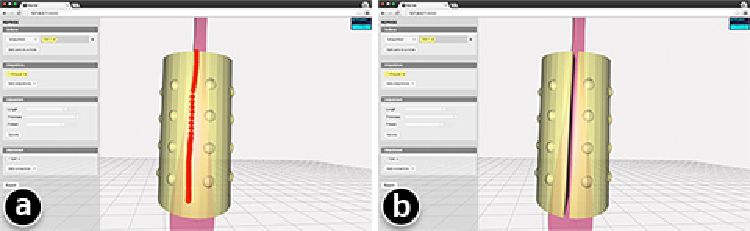
\includegraphics[width=0.75\textwidth]{figures/reprise_split_v1.pdf}
  \caption{Reprise provides a simple technique to split an adaptation in halves so an object, such as this fork, can be put inside a wrapper (Figure~\ref{fig:reprise_wrapper_results}a).}~\label{fig:reprise_split}
\end{figure}

\begin{figure}[h!]
  \vskip 8pt
  \centering
  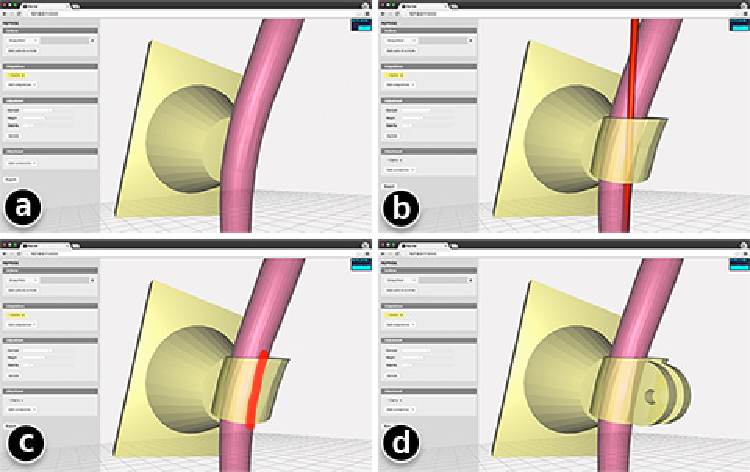
\includegraphics[width=0.75\textwidth]{figures/reprise_pipeclamp_v1.pdf}
  \caption{A pipe clamp, provided by Reprise, attaches the generated stand (a) to the object. Clicking on the object places the pipe (b). Another stroke cuts it open and adds a pair of clamps (cd).}~\label{fig:reprise_pipeclamp}
\end{figure}

\begin{figure}[h!]
  \vskip 8pt
  \centering
  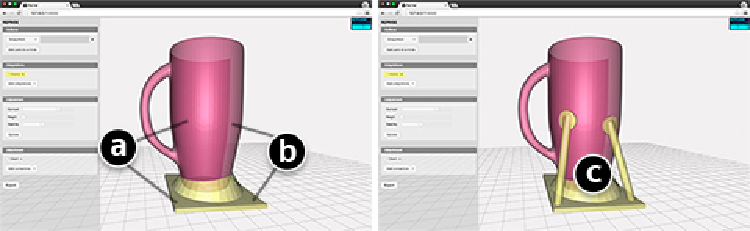
\includegraphics[width=0.75\textwidth]{figures/reprise_beams_v1.pdf}
  \caption{Beams can further support the object for an adaptation. To generate one, simply select a point on the object and another point on the adaptation.}~\label{fig:reprise_beams}
\end{figure}

In some cases, part of an object is not accessible or should not be occluded by the adaptations, such as a phone's screen. Reprise allows a user to specify which part of the object should be excluded when generating adaptations. As shown in Figure~\ref{fig:reprise_inaccessible}a, the phone's screen is marked as inaccessible (red), and accordingly the generated handle avoids covering the screen area (Figure~\ref{fig:reprise_inaccessible}b).

\begin{figure}[h!]
  \vskip 7pt
	\centering
	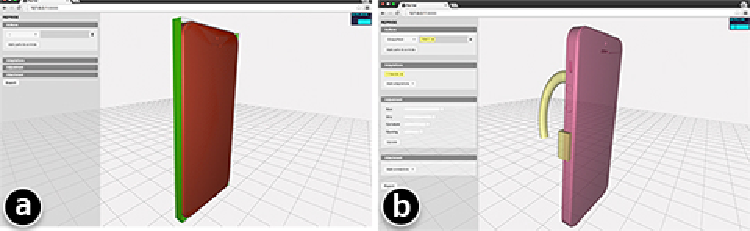
\includegraphics[width=0.75\textwidth]{figures/reprise_inaccessible_v1.pdf}
	\caption{As the phone's screen is marked as inaccessible (red) by an adaptation, the generated handle avoids covering that area.}~\label{fig:reprise_inaccessible}
\end{figure}

\subsection{Implementation, Measurement and Fabrication}
Reprise was implemented using JavaScript with three.js\footnote{\url{http://threejs.org/}} and OpenJSCAD\footnote{\url{http://openjscad.org/}}. The tool can run readily inside a modern browser. Reprise curates a 3D model repository of common household items and hand tools; alternatively, it also uses Skanect\footnote{\url{http://skanect.occipital.com/}} and the Makerbot Digitizer \footnote{\url{http://store.makerbot.com/digitizer}} for digitalizing objects. The spray bottle in Figure~\ref{fig:reprise_clutch} was scanned using the Skanect system.

For some adaptations, users might need to measure the hand or finger sizes of the person. Reprise comes with a simple measuring tool (Figure~\ref{fig:reprise_hand_measuring}) that can be printed (and cut) on a piece of paper, or made with a laser cutter. The hand measuring part is based on a method for determining the size for a golf glove\footnote{\url{http://www.jumbomax.com/sizing/}}. The finger part is based-on standard ring-size metrics.

\begin{figure}[h!]
\vskip 7pt
  \centering
  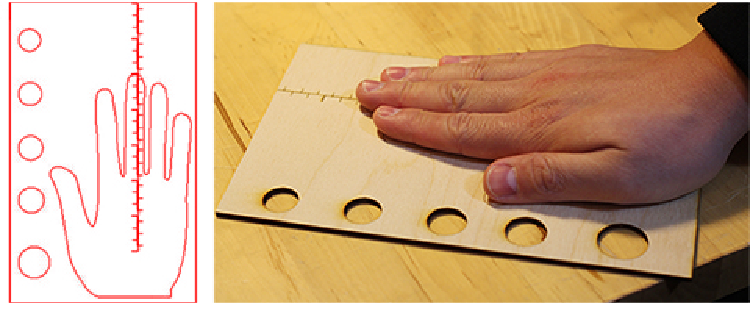
\includegraphics[width=0.9\textwidth]{figures/reprise_hand_measuring_v1.pdf}
\caption{Reprise also provides an SVG file for making a measuring tool for adaptations that require fitting users' hand or fingers. This one shown above was laser cut.}~\label{fig:reprise_hand_measuring}
\end{figure}

For fabrication, we used material with various softness, ranging from regular PLA, to SemiFlex\footnote{\url{http://www.ninjaflex3d.com/products/semiflex/}}, Nylon-based\footnote{\url{http://www.graphene3dlab.com/}} or NinjaFlex\footnote{\url{http://www.ninjaflex3d.com/products/ninjaflex-filaments/}}. All the results--as we demonstrate below--were fabricated using an inexpensive Printrbot Play 3D printer\footnote{\url{https://printrbot.com/shop/assembled-printrbot-play/}}.

%\hl{Currently Reprise only deals with geometry; in the future it would be interesting to incorporate some consideration of material, such as recommending what filament to use for a given kind of adaptation.} 

\section{Results and Validation Through Replication}
Compared to traditional CAD tools where models are mostly created from scratch, Reprise has integrated application domain specific knowledge that allows users to specify, generate and customize adaptations at a higher level. While there may remain some usability issues with our tool, this application domain targeted approach clearly allows adaptations to be specified much more easily than trying to create them as unstructured arbitrary geometry in a general-purpose tool.  However, this ease of use can come at a price, and this raises the important issue of whether the tool can create a wide range of objects to cover an interesting and useful space. To answer this more difficult question, we validate Reprise by focusing on its breadth of expressiveness.  In particular, we used it to replicate a wide spread of existing adaptation examples. This demonstrates the potential for Reprise to support the full range of adaptations that are demonstrably useful in the real world.

% We chose to perform this exercise as an expert user, to overcome the limit of a laboratory study where each participant only has a limited time to explore or iterate a few different adaptation designs.

Specifically, we chose to replicate representative cases from different `cells' in the design space of adaptations (Figure~\ref{fig:reprise_design_space}). Below we showcase our results, discuss issues that arose during the process, and identify cases where Reprise is not yet able to generate the adaptations, which suggest opportunities for future work.

% Due to the time-consuming and iterative nature of 3D printing, the time frame of a typical usability study would limit the number of adaptations that can be designed and fabricated. As such, we chose to

\textbf{\#1 Wrappers/Extensions}
As shown in Figure~\ref{fig:reprise_wrapper_results}, Reprise was able to replicate all the four wrapper/extension examples in the design space. The virtual hand was effective in positioning the wrapper at the right place on the objects. However, in the case of the cutter handle, we found that the simple cylindrical structures did not fully conform to the curvature of the handles (Figure~\ref{fig:reprise_wrapper_results}d). A new feature for future work would be to `curve' the wrapper so that it can better represent the original geometry of the object.

% As shown in Figure~\ref{fig:reprise_wrapper_results}, Reprise replicated the gripper for a fork (Figure~\ref{fig:reprise_wrapper_results}a), the extension for a zipper pull (Figure~\ref{fig:reprise_wrapper_results}b), and the tennis ball opener (Figure~\ref{fig:reprise_wrapper_results}c), all of which we fabricated  using either Nylon-based or Ninja Flex soft material. The cutter handle wrapper (Figure~\ref{fig:reprise_wrapper_results}d) supports clutching and thus meets the Figure~\ref{fig:reprise_design_space}-E1 category; however its purpose is different from the existing example (Figure~\ref{fig:reprise_wrapper_results}d inset), which is specifically designed for safety concerns.

\begin{figure}[h!]
  \centering
  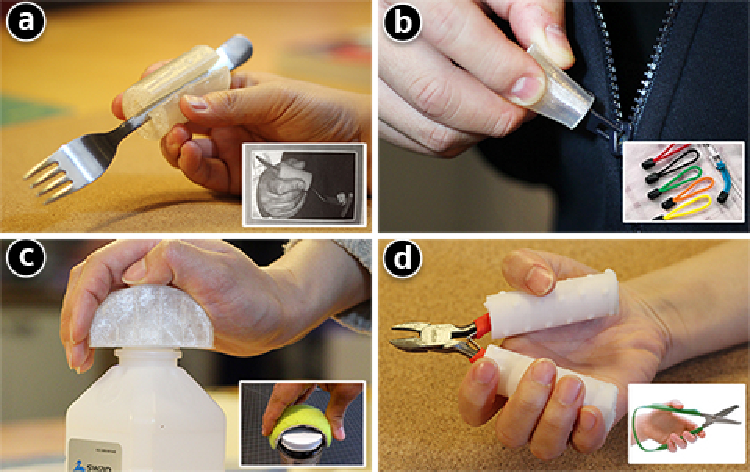
\includegraphics[width=0.75\textwidth]{figures/reprise_wrapper_results_v1.pdf}
  \caption{Replicated wrapper/extension examples. Ninjaflex was used for the fork wrapper (a), zipper handle extension (b), and the bottle lid wrapper (c). Nylon-based soft material was used for the cutter. }~\label{fig:reprise_wrapper_results}
\end{figure}


\textbf{\#2 Handles}
All types of handle examples in the design space were replicated using Reprise (Figure~\ref{fig:reprise_handle_results}). Reprise allows users to explore different handle designs, such as making a `closed loop' for holding and turning a key (Figure~\ref{fig:reprise_handle_results}c), or half-open for easier placement of the hand when holding a phone (Figure~\ref{fig:reprise_handle_results}a) or pulling open a cabinet door (Figure~\ref{fig:reprise_handle_results}b). 

A single handle can be used to stabilize the grip of a pen (Figure~\ref{fig:reprise_combine_adaptations}a) while it is also possible to combine multiple handles to match different fingers (Figure~\ref{fig:reprise_handle_results}d). In particular, for fingers, initially we found it really hard to specify a fixed spatial relationship between them and the handles, as their position and orientation could vary from time to time while holding an object. Later we found that using soft material could mitigate this problem, as its deformable nature offers a range of adjustable configurations. Although Reprise operates at the geometry level, it is possible, as a future step, to fine tune the geometry of a handle as a way to `program' its range of configuration when printed with soft material.
\vskip 5pt
% All types of handle examples in the design space were replicated using Reprise (Figure~\ref{fig:reprise_handle_results}). Reprise allows users to explore different handle designs, such as making a `closed loop' for holding and turning a key (Figure~\ref{fig:reprise_handle_results}c), or half-open for easier placement of the hand when holding a phone (Figure~\ref{fig:reprise_handle_results}a) or pulling open a cabinet door (Figure~\ref{fig:reprise_handle_results}b). Multiple handles can also be combined to match with different fingers (Figure~\ref{fig:reprise_handle_results}d).

%\vskip 2pt

\begin{figure}[h!]
  \centering
  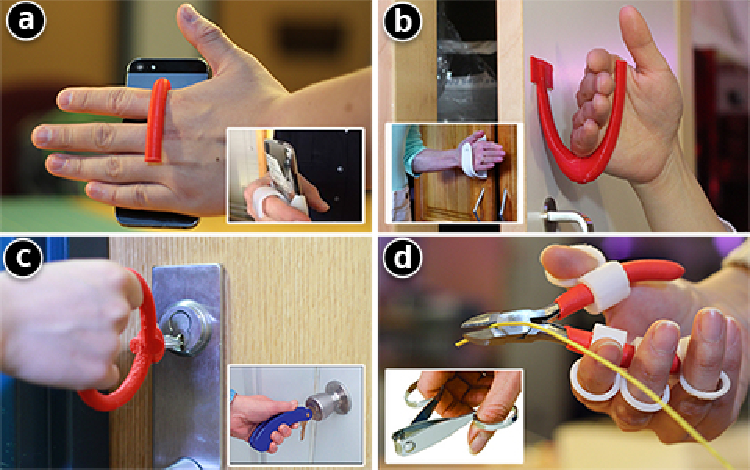
\includegraphics[width=0.75\textwidth]{figures/reprise_handle_results_v1.pdf}
  \caption{Replicated handle examples.}~\label{fig:reprise_handle_results}
\end{figure}

\textbf{\#3 Levers}
Figure~\ref{fig:reprise_lever_results} shows Reprise' replication of levers. One current limitation we found is that Reprise can only generate levers where part of the existing object has a degree of freedom to be rotated or squeezed. In the future we plan to explore other use cases of a lever, such as for clamping (Figure~\ref{fig:reprise_design_space}-A3) or separating (Figure~\ref{fig:reprise_design_space}-C3) static objects.
\vskip 3pt

% For rotation, we created a lever for a small cylindrical light switch (Figure~\ref{fig:reprise_lever_results}a), in spirit similar to the faucet design in Figure~\ref{fig:reprise_design_space}-D3. We also adapted a spray bottle to replicate the existing example (Figure~\ref{fig:reprise_lever_results}b). Currently Reprise can only generate levers where part of the existing object has a degree of freedom to be rotated or clutched. In the future we plan to explore other use cases of a lever, such as for clamping (Figure~\ref{fig:reprise_design_space}-A3) or separating (Figure~\ref{fig:reprise_design_space}-C3) static objects. 

\begin{figure}[h!]
\vskip 5pt
  \centering
  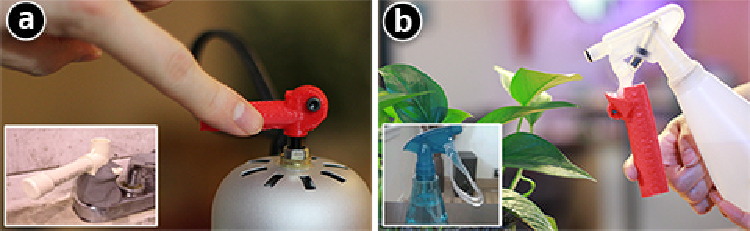
\includegraphics[width=0.75\textwidth]{figures/reprise_lever_results_v1.pdf}
  \caption{Replicated lever examples.}~\label{fig:reprise_lever_results}
\end{figure}

\textbf{\#4 Anchors/Stands}
Besides the aforementioned cutter, we also replicated two other anchor/stand examples as shown in Figure~\ref{fig:reprise_anchor_results}. When making these examples, we often found it necessary to add extra fasteners or support structures, such as the pipe clamp for the cutter (Figure~\ref{fig:reprise_anchor_results}a) and the supporting beams for the mug and the sharpie anchor (Figure~\ref{fig:reprise_anchor_results}bc). Rather than adding them as a follow-up step, future work could integrate these components parametrically as part of the generated adaptation.

% Besides the aforementioned cutter, we also replicated the stabilized cup design (Figure~\ref{fig:reprise_anchor_results}b) and an anchor for holding a sharpie (which is in spirit similar to the Belliclamp device in Figure~\ref{fig:reprise_design_space}-D4). Both our sharpie anchor and the Belliclamp also involve multiple actions--joining/separating objects by means of pushing, pulling or rotation.

\begin{figure}[t]
  \centering
  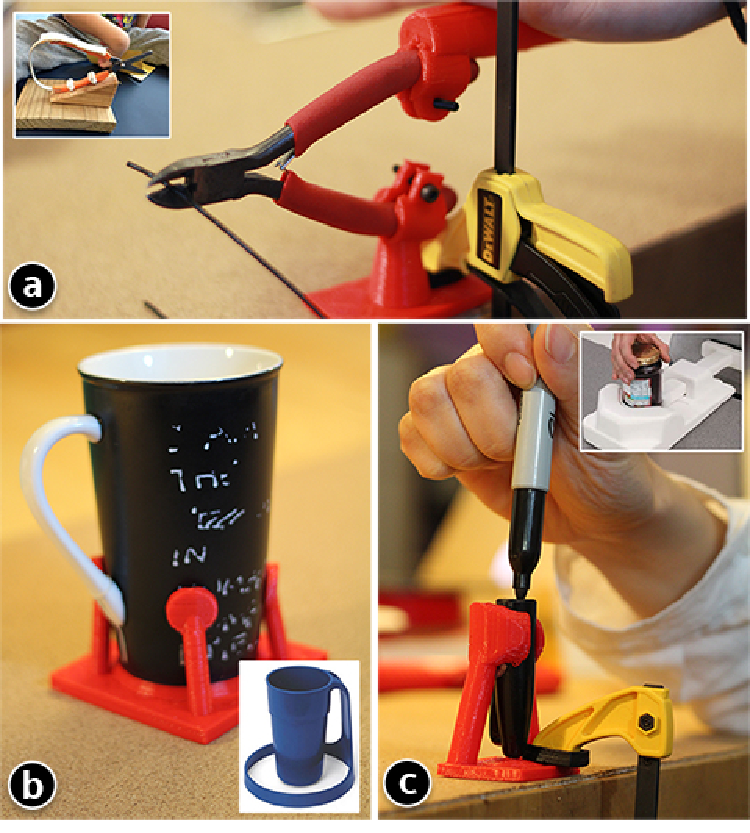
\includegraphics[width=0.7\textwidth]{figures/reprise_anchor_results_v1.pdf}
  \caption{Replicated anchor/stand examples.}~\label{fig:reprise_anchor_results}
\end{figure}

\textbf{\#5 Guides}
Inspired by the drilling guide example (Figure~\ref{fig:reprise_design_space}-C5), we used Reprise to generate similar structures for guiding a key towards a lock (Figure~\ref{fig:reprise_guide_results}a) and putting a sharpie back into its cap (Figure~\ref{fig:reprise_guide_results}b). We did not replicate the remote control example as it stands (Figure~\ref{fig:reprise_design_space}-B5), as it seems simple enough to be made with paper, and further it sacrificially occludes other buttons. Instead, we opted for an alternate design--an extension on the button that makes it a larger target for pressing (Figure~\ref{fig:reprise_wrapper}b). It is interesting to see that in this case an extension can also serve as a guide, which suggests the possibility of `remixing' categorically different adaptation strategies.


% Inspired by the drilling guide example (Figure~\ref{fig:reprise_design_space}-C5), we used Reprise to generate similar structures for guiding a key towards the lock (Figure~\ref{fig:reprise_guide_results}a) and putting a sharpie back into its cap (Figure~\ref{fig:reprise_guide_results}b). We did not replicate the remote control example (Figure~\ref{fig:reprise_design_space}-B5), as there seems to be an easier solution--cutting and pasting pieces of paper\footnote{However, to avoid occluding other buttons, Reprise can generate an alternate design--an extension on the button that makes it a larger target for pressing (Figure~\ref{fig:reprise_wrapper}b)}. Reprise currently only guides linear motion; in the future it should be possible to explore how to generate guides for other types of motion, such as a guide for turning faucets to get (only) mildly warm water.

\begin{figure}[h!]
  \vskip 5pt
  \centering
  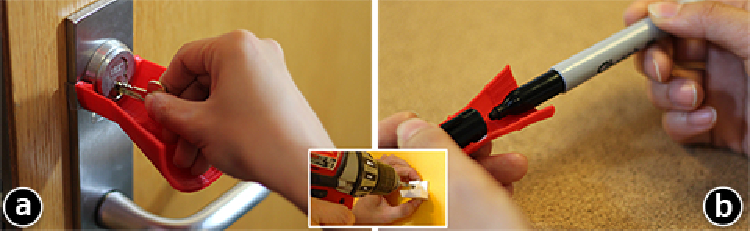
\includegraphics[width=0.75\textwidth]{figures/reprise_guide_results_v1.pdf}
  \caption{Replicated guide examples.}~\label{fig:reprise_guide_results}
\end{figure}

One limitation we found is that Reprise currently only guides linear motion; in the future it should be possible to explore how to generate guides for other types of motion, such as a guide for turning faucets to get (only) mildly warm water.


\section{Discussion and Summary of Designing Adaptations}
Based on our exploration of the design space, tool integration and fabricated results of adaptations, we now discuss existing issues, limitations and potential future work.

\textbf{Combining different adaptations}
With Reprise, it is also possible to combine different adaptation strategies. Figure~\ref{fig:reprise_combine_adaptations} shows a series of sharpie adaptations generated by Reprise, ranging from a handle for holding (Figure~\ref{fig:reprise_combine_adaptations}a), the aforementioned guide (Figure~\ref{fig:reprise_combine_adaptations}b) and anchor (Figure~\ref{fig:reprise_combine_adaptations}c), and finally, a combination of the three (Figure~\ref{fig:reprise_combine_adaptations}d). Our current approach is to incrementally add new adaptation with the previous ones considered as part of the object. However, the ordering of addition could cause adaptations to conflict with one another. For example, adding a handle might make the sharpie no longer fit in the guide installed earlier. Future work could optimize the order of adding multiple adaptations to reduce conflict, or updating existing adaptations as new ones are added.

\begin{figure}[h!]
  \centering
  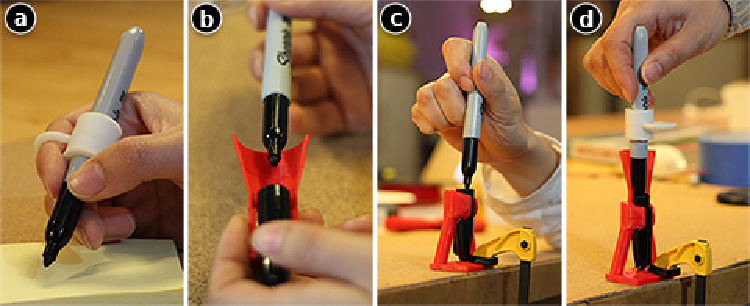
\includegraphics[width=1\textwidth]{figures/reprise_combine_adaptations_v1.pdf}
  \caption{Combining multiple adaptations: a handle (a), a guide (b) and an anchor (c) can be combined into one (super) adaptation (d).}~\label{fig:reprise_combine_adaptations}
\end{figure}


\textbf{Expanding the feedback loop for customization}
Rather than just taking the original object as input, future work could enable a more iterative approach where a printed piece of adaptation can be fed into the system to let the user further customize it. Prior work, such as ModelCraft \cite{song2006modelcraft} could potentially be extended here to let the user annotate printed results for the next design iteration.

\textbf{Scaling up reprise to adapt larger objects}
Most of the objects Reprise adapted so far are hand-sized items or tools. In future it would be interesting to explore larger scaled adaptations, such as making a bath tub safer to walk in/out, or making room entrances or stairwells more accessible. The challenges are two-fold: how to scale up the current design workflow to incorporate large objects, and how to go beyond the usual volume of 3D printers to fabricate the adaptations.

% \textbf{Evaluating the Usability and Learnability of Reprise}
% We designed Reprise with a goal in mind to make the process as simple as possible. Indeed, Reprise dispenses with low-level mesh manipulation--users specify types of actions, generate adaptation models, adjust the design parameters and add attachment aids, all in a few mouse clicks and drags. However, despite the intentional simplicity, Reprise still presents itself as a 3D modeling tool wherein each step does require certain level of understanding in 3D geometry. Future work could test Reprise with users who have little or no 3D modeling experience to reveal whether and where they have difficulty with the design workflow.

\textbf{Combining hand-making and digital fabrication}
Although we designed Reprise for 3D printing, we believe it may work best as a tool that complements existing hand-making approachs, rather than replacing them. Hand-making can capture users' intuition and creativity (even though the outcome is still limited by the materials available and the users' making skill). Future work could transform Reprise's workflow to incorporate or augment handmade prototypes, such as using 3D printed fasteners to connect handmade parts, or to serve as components that require higher functional precision.

\textbf{Using vision-based sensors to capture object usage}
As we designed the virtual hand for specifying different ways of grasping, we realized the possibility of an alternate approach where the person can use an RGB+depth camera (e.g., Kinect) to show their grip by performing it. This seems a more natural way to express one's difficulty with objects. Further, the person's hand shape might also be captured by first gripping a piece of clay \cite{buehler2014coming} and then digitalizing it. Although compelling, this type of vision-based approach has inherent issues, such as the imprecision of the sensors and the general difficulty in reconstructing the captured data into high-fidelity 3D models.

% \textbf{Exploring Mechanism as a New Adaptation Strategy}
% Mechanism provides a simple mechanical system for applying motion to certain objects, usually by replacing the original motion with new type of motion favorable by the users. Figure XXa shows a design sketch of a cam mechanism applied on a spray bottle so that users with difficulty squeezing can instead turning a crank to press the spraying handle. Figure XXb shows a universal joint attached to a screw driver, which accommodates a wider range of angle and hand posture when applying the rotation motion. Figure XXc is simple clutch mechanism as an alternate way of holding an object tight.

%\xac{
%
%* adaptations that handle a range of objects rather than a specific object
%
%* human creativity + machine intelligence/precision
%
%* combining 3d printing and material that is readily available
%
%  adapting large scale objects?
% 
% large scale: https://www.youtube.com/watch?v=CKl_3mnj3dM
%}
%
%\xac{
%* tying shoelaces
%
%* clothes buttons
%}


In my work thus far, either extending or adapting existing objects allows for incremental `delta' for transforming the real world, as their functionality is somewhat dependent on the objects they are attached to. For a non-incremental approach, where brand-new objects are created from scratch, the objects we create will often end up physically interacting with others. A bookshelf will be used to put on books. A chair will be sit on. A step stool will stood upon. How can facilitate the design process so that objects like these can function properly and reliably with real world objects they will be used with. My next chapter proposes a design tool to support users in conducting such fuctionally aware design tasks.